\documentclass{report}
\usepackage[margin=1in, paperwidth=8.5in, paperheight=11in]{geometry}
%Math packages%
\usepackage{amsmath}
\usepackage{amsthm}
%Spacing%
\usepackage{setspace}
\onehalfspacing
%Lecture number%
\newcommand{\lectureNum}{4}
%Variables - Date and Course%
\newcommand{\curDate}{January 11, 2017}
\newcommand{\course}{MATH 239}
\newcommand{\instructor}{Peter Nelson (substitute)}
%Defining the example tag%
%\theoremstyle{definition}%
\newtheorem{ex}{Example}[section]
%Setting counter given the lecture number%
\setcounter{chapter}{\lectureNum{}}
%Package for drawing graphs%
\usepackage{tikz}
\usepackage{verbatim}
\usetikzlibrary{arrows}

\begin{document}
%Note title%
\begin{center}
\begin{Large}
\textsc{\course{} | Lecture \lectureNum{}}
\end{Large}
\end{center} 
\noindent \textit{Bartosz Antczak} \hfill
\textit{Instructor: \instructor{}} \hfill
\textit{\curDate{}}
\rule{\textwidth}{0.4pt}

% Actual Notes%
\subsubsection{Recall from last lecture | Handshaking Theorem}
In a graph $G = (V, E)$
$$\displaystyle \sum_{v\in V} \mathrm{deg}(v) = 2 \vert E \vert$$
A corollary that stems from this states that the average degree of a vertex in $ G = (V, E)$ is $\displaystyle \frac{2 \vert E \vert}{\vert V \vert}$
\subsubsection{Definition: k-regular}
A graph is \textbf{k-regular} if every vertex in it has degree $k$. Some examples include
\begin{itemize}
\item the Petersen graph (3-regular)
\item the complete graph ($K_n$ is $(n - 1)$-regular)
\item cycle graphs ($C_n$ is 2-regular for all $n$)
\end{itemize}
By the handshaking theorem, if $G = (V, E)$ is a k-regular graph, then
$$\vert E \vert = \sum_{v \in V} \mathrm{deg}(v) = \frac{1}{2}k \vert V \vert$$
For instance, using this equation, the complete graph $K_n$ is $(n-1)$-regular and has $n$ vertices, so 
$$\vert E(K_n)\vert = \frac{1}{2}n(n-1) = {n \choose 2}$$
\subsubsection{Definition: n-cube}
The \textbf{n-cube}, $Q_n$ is defined by
\begin{itemize}
\item $V(Q_n) =$ \{binary string of length $n$\}; $\vert V(Q_n) \vert$ = $2^n$
\item $E(Q_n) =$ \{pairs of strings that differ in exactly one position\}; $\vert E(Q_n) \vert$ = $n \cdot 2^{n-1}$
\end{itemize}
To better visualize this, shown are a 1-cube and 2-cube graph:
%n-cube graphs%
\begin{center}
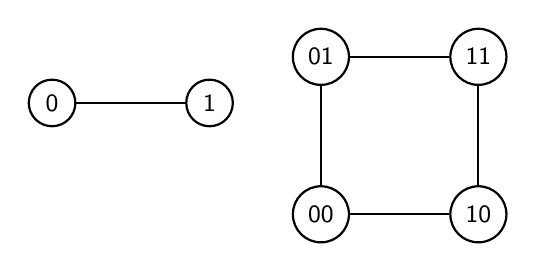
\begin{tikzpicture}[-,auto,node distance=2cm,
                    thick,main node/.style={circle,draw,font=\sffamily\small}]
  %1-cube%
  \node[main node] (1) {0};
  \node[main node] (2) [right of=1] {1};
  %2-cube%
  \node[main node] (3) [below right of=2]{00};
  \node[main node] (4) [above of=3]{01};
  \node[main node] (5) [right of=3]{10};
  \node[main node] (6) [above of=5]{11}; 
  \path[every node/.style={font=\sffamily\small}]
    (1) edge node [left] {} (2)
    (3) edge node [right] {} (4)
	    edge node [above] {} (5)
	(6) edge node [right] {} (4)
		edge node [right] {} (5);
\end{tikzpicture}
\end{center}
\section{Paths and Walks}
\underline{Recall} the path on $n$ vertices $P_n$ has vertex set $\{1, \cdots, n\}$ and edge set $\{\{i, i+1\} \,\vert\, 1 \leq i < n\}$.\\
A \textbf{path} from $u$ to $v$ in a graph is a sequence $u_0, e_1, u_1, e_2, \cdots , u_{k-1}, e_k, v_k$ where
\begin{itemize}
\item $u_0 = u$ and $u_k = v$
\item For $1 \leq i \leq k$, $u_i$ are distinct vertices of $G$ and $e_i$ is an edge of $G$ from $u_{i-1}$ to $u_i$
\end{itemize}
Shown is an example of a simple path (note that $u_i \neq u_j$ for all $i \neq j$):
%Path example graph%
\begin{center}
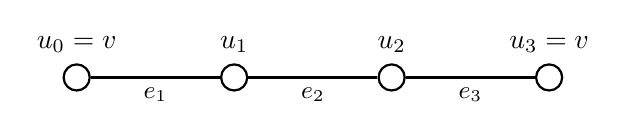
\begin{tikzpicture}[-,auto,node distance=2cm,
                    thick,main node/.style={circle,draw,font=\sffamily\small}]
  %1-cube%
  \node[main node] (1) [label={$u_0=v$}]{};
  \node[main node] (2) [right of=1][label={$u_1$}]{};
  \node[main node] (3) [right of=2][label={$u_2$}]{};
  \node[main node] (4) [right of=3][label={$u_3=v$}]{};
  \path[every node/.style={font=\sffamily\small}]
    (1) edge node [below] {$e_1$} (2)
    (2) edge node [below] {$e_2$} (3)
    (3) edge node [below] {$e_3$} (4);        
\end{tikzpicture}
\end{center}

\noindent A \textbf{walk} from $u$ to $v$ in $G$ is defined in the same way as a path, except we drop the requirement that the vertices are distinct.\\
A good distinction between a walk and a path is that if there exists a walk from $u$ to $v$ and from $v$ to $w$, then there exists one from $u$ to $w$; but the same isn't true for a path, because the path from $v$ to $w$ may intersect with some vertices from the path from $u$ to $v$, causing not all vertices being distinct, ergo not a path (\textit{however}, we can convert it to a path | this is proven in the corollary below).
\subsection{Proposition about Paths}
\textit{If there is a walk from $u$ to $v$ in $G$, then there is a path from $u$ to $v$.}
\\\\
\textbf{Proof:} Let $u = u_0, e_1, u_1, e_2, \cdots, e_k, u_k$ be the shortest walk from $u$ to $v$. If $u_0, u_1, \cdots, u_k$ are distinct, then the walk is a path and there is nothing to prove. Otherwise, $u_i = u_j$ for some $i < j$. But then $u = u_0, e_1, u_1, e_2, \cdots, u_i = u_j, e_{j+1}, u_{j+1}, \cdots, e_k, u_k$ is a shorter walk (a.k.a. has fewer edges) from $u$ to $v$, which is a contradiction. Thus, a walk can always be converted to a path.
\subsubsection{Corollary}
\textit{If $u$, $v$, $w$ are vertices of a graph $G$ and there is a path from $u$ to $v$ and a path from $v$ to $w$, then there is a path from $u$ to $v$.}\\\\
\textbf{Proof:} Combine both paths from $u$ to $v$ and $v$ to $w$. If this combination is also a path, then we're done. If it's a walk, then the previous proposition shows that all walks can be converted to paths. Thus, there is a path from $u$ to $v$.
%END%
\end{document}